\documentclass[]{article}

% definitions
\def\D{\partial}

\def\solidline{{$\textcolor{blue}{\overline{\hskip 0.5cm}}\ $}}
\def\dashedline{{$\textcolor{red}{\overline{\hskip 0.1cm}\ \overline{\hskip 0.1cm}\ \overline{\hskip 0.1cm}\ }$}}
\def\dashdottedline{$\overline{\hskip 0.1cm}\ \overline{\hskip 0.03cm}\ \overline{\hskip 0.1cm}\ $}
\def\dottedline{$\overline{\hskip 0.04cm}\ \overline{\hskip 0.04cm}\ \overline{\hskip 0.04cm}\ $}

\usepackage{amsmath,amssymb,amsthm}
\newtheorem{thm}{Theorem}
\usepackage{lettrine}
\usepackage{amsfonts}
\usepackage[pdftex]{graphicx}
\usepackage[latin1]{inputenc}
\usepackage{epstopdf}
\usepackage{hyperref}
\usepackage{placeins}
\usepackage{bigints}
\usepackage{gensymb}
\usepackage{float}
\usepackage{color}
\usepackage{graphicx}
\usepackage{graphics}
\usepackage[hmarginratio=1:1,top=25mm,columnsep=20pt]{geometry}
\usepackage[font=it]{caption}
\usepackage{paralist}
\usepackage{multicol}
\usepackage{lettrine}
\usepackage[nodayofweek]{datetime}
\usepackage{centernot}
\usepackage{ mathrsfs }
\usepackage{textcomp}
\usepackage{color}
%\usepackage{listings}
\usepackage{setspace}
\usepackage{xcolor}
\usepackage{subcaption}
\usepackage{color}
\usepackage[procnames]{listings}
\usepackage{setspace}
\usepackage{palatino}
\usepackage{multirow}

\renewcommand{\lstlistlistingname}{Code Listings}
\renewcommand{\lstlistingname}{Code Listing}
\definecolor{gray}{gray}{0.5}
\definecolor{green}{rgb}{0,0.5,0}
\definecolor{lightgreen}{rgb}{0,0.7,0}
\definecolor{purple}{rgb}{0.5,0,0.5}
\definecolor{darkred}{rgb}{0.5,0,0}
\lstnewenvironment{python}[1][]{
\lstset{
language=python,
basicstyle=\ttfamily\small\setstretch{1},
stringstyle=\color{green},
showstringspaces=false,
alsoletter={1234567890},
otherkeywords={\ , \}, \{},
keywordstyle=\color{blue},
emph={access,and,as,break,class,continue,def,del,elif,else,%
except,exec,finally,for,from,global,if,import,in,is,%
lambda,not,or,pass,print,raise,return,try,while,assert},
emphstyle=\color{orange}\bfseries,
emph={[2]self},
emphstyle=[2]\color{gray},
emph={[4]ArithmeticError,AssertionError,AttributeError,BaseException,%
DeprecationWarning,EOFError,Ellipsis,EnvironmentError,Exception,%
False,FloatingPointError,FutureWarning,GeneratorExit,IOError,%
ImportError,ImportWarning,IndentationError,IndexError,KeyError,%
KeyboardInterrupt,LookupError,MemoryError,NameError,None,%
NotImplemented,NotImplementedError,OSError,OverflowError,%
PendingDeprecationWarning,ReferenceError,RuntimeError,RuntimeWarning,%
StandardError,StopIteration,SyntaxError,SyntaxWarning,SystemError,%
SystemExit,TabError,True,TypeError,UnboundLocalError,UnicodeDecodeError,%
UnicodeEncodeError,UnicodeError,UnicodeTranslateError,UnicodeWarning,%
UserWarning,ValueError,Warning,ZeroDivisionError,abs,all,any,apply,%
basestring,bool,buffer,callable,chr,classmethod,cmp,coerce,compile,%
complex,copyright,credits,delattr,dict,dir,divmod,enumerate,eval,%
execfile,exit,file,filter,float,frozenset,getattr,globals,hasattr,%
hash,help,hex,id,input,int,intern,isinstance,issubclass,iter,len,%
license,list,locals,long,map,max,min,object,oct,open,ord,pow,property,%
quit,range,raw_input,reduce,reload,repr,reversed,round,set,setattr,%
slice,sorted,staticmethod,str,sum,super,tuple,type,unichr,unicode,%
vars,xrange,zip},
emphstyle=[4]\color{purple}\bfseries,
upquote=true,
morecomment=[s][\color{lightgreen}]{"""}{"""},
commentstyle=\color{red}\slshape,
literate={>>>}{\textbf{\textcolor{darkred}{>{>}>}}}3%
         {...}{{\textcolor{gray}{...}}}3,
procnamekeys={def,class},
procnamestyle=\color{blue}\textbf,
framexleftmargin=1mm, framextopmargin=1mm, frame=shadowbox,
rulesepcolor=\color{blue},#1
}}{}


%%%%% Titling
\usepackage[compact]{titlesec}
\newcommand{\overbar}[1]{\mkern 1.5mu\overline{\mkern-1.5mu#1\mkern-1.5mu}\mkern 1.5mu}

\newenvironment{corollary}[1]{\par\noindent\underline{Corollary:}\space#1}{}
\newenvironment{lemma}[1]{\par\noindent\underline{Lemma:}\space#1}{}
\newenvironment{theorem}[1]{\par\noindent\underline{Theorem:}\space#1}{}
\newenvironment{claim}[1]{\par\noindent\underline{Claim:}\space#1}{}
\newenvironment{proposition}[1]{\par\noindent\underline{Proposition:}\space#1}{}
\newenvironment{claimproof}[1]{\par\noindent\underline{Proof:}\space#1}{\hfill\ensuremath{\square}}

\include{pythonlisting}

% ------
% Header/footer
\usepackage{fancyhdr}
	\pagestyle{fancy}
	\fancyhead{}
	\fancyfoot{}
	\fancyhead[C]{Surrogate Optimization Toolbox in Python (pySOT) - 0.1.15 $\bullet$ Tutorial $\bullet$ David Eriksson, David Bindel, Christine Shoemaker $\bullet$ \today}
	\fancyfoot[RO,LE]{\thepage}

%%% ---- MATLAB CODE ---- %%%

\definecolor{Blue}{rgb}{0.1,0.1,0.3}
\hypersetup{colorlinks=true,linkcolor=Blue,citecolor=Blue,urlcolor=Blue}

\definecolor{listinggray}{gray}{0.9} 
\definecolor{lbcolor}{rgb}{0.9,0.9,0.9}
\definecolor{dorange}{rgb}{1.000000,0.549020,0.000000}
\definecolor{lblue}{rgb}{0.529412,0.807843,0.980392}
\lstset{escapeinside={<@}{@>}}


\definecolor{orange}{rgb}{1,0.5,0}
\DeclareMathOperator{\sgn}{sgn}
\DeclareMathOperator{\tr}{tr}
\DeclareMathOperator{\argmax}{argmax}
\DeclareMathOperator{\X}{\mathcal{X}}
\DeclareMathOperator{\Y}{\mathcal{Y}}
\DeclareMathOperator{\Z}{\mathbb{Z}}
\DeclareMathOperator{\Fx}{\mathcal{F}_{\X}}
\DeclareMathOperator{\Fy}{\mathcal{F}_{\Y}}
\DeclareMathOperator{\Fz}{\mathcal{F}_{\Z}}
\DeclareMathOperator{\Nc}{\mathcal{N}}
\DeclareMathOperator{\Rc}{\mathcal{R}}
\DeclareMathOperator{\B}{\mathcal{B}}
\DeclareMathOperator{\C}{\mathbb{C}}
\DeclareMathOperator{\Rb}{\mathbb{R}}
\DeclareMathOperator{\Sb}{\mathcal{S}}
\DeclareMathOperator{\N}{\mathbb{N}}
\DeclareMathOperator{\Q}{\mathbb{Q}}
\DeclareMathOperator{\limn}{\lim\limits_{n \to \infty}}
\DeclareMathOperator{\limm}{\lim\limits_{m \to \infty}}
\DeclareMathOperator{\R}{Re}
\DeclareMathOperator{\I}{Im}
\DeclareMathOperator{\spann}{span}
\newcommand*{\QED}{\hfill\ensuremath{\square}}%

%%%% Title
\title{\vspace{-15mm}%
	\fontsize{18pt}{10pt}\selectfont
	\textbf{Surrogate Optimization Toolbox (pySOT) - 0.1.15 \\ Tutorial}
	}	
\author{%
	\Large\textsc{David Eriksson} \\[2mm]
	\Large\textsc{David Bindel} \\[2mm]
	\Large\textsc{Christine Shoemaker} \\[2mm]
		\normalsize	Cornell University \\
	\normalsize Center for Applied Mathematics \\
	\normalsize	dme65@cornell.edu \\ 
	}
\date{\today}

\begin{document}
\fontsize{12}{14}\rm

\maketitle
\thispagestyle{fancy}
\tableofcontents
\newpage

\section{Change history:}
\begin{itemize}

\item (\textbf{0.1.15})
\begin{itemize}
\item Added an example test\_subprocess\_files that shows how to use pySOT in case the objective function needs to read the input from a textfile
\end{itemize}

\item (\textbf{0.1.14}) 
\begin{itemize}
\item Updated the Tutorial to reflect the changes for the last few months
\item Simplified the object creation from strings in the GUI by importing directly from the namespace.
\end{itemize}

\item (\textbf{0.1.13}) 
\begin{itemize}
\item Allowed to still import the rest of pySOT when PySide is not found. In this case, the GUI will be unavailable.
\end{itemize}

\item (\textbf{0.1.12}) 
\begin{itemize}
\item The capping can now take in a general transformation that is used to transform the function values. Default is median capping.
\item The Genetic Algorithm now defaults to initialize the population using a symmetric latin hypercube design
\item DYCORS uses the remaining evaluation budget to change the probabilities after a restart instead of using the total budget 
\end{itemize}

\item (\textbf{0.1.11}) 
\begin{itemize}
\item Fixed a bug in the capped response surface
\item pySOT now internally works on the unit hypercube
\item The distance can be passed to the RBF after being computed when generating candidate points so it is not computed twice anymore
\item Fixed some bugs in the candidate functions
\item GA and Multi-Search gradient perturb the best solution in the case when the best solution is a previously evaluated point
\item Added an additional test for the multi-search strategy
\end{itemize}

\item (\textbf{0.1.10}) 
\begin{itemize}
\item README.md not uploaded to pypi which caused the pip install to fail
\end{itemize}

\item (\textbf{0.1.9}) 
\begin{itemize}
\item Fixed a bug in the merit function and several bugs in the DYCORS strategy
\item Added a DDS candidate based strategy for searching on the surrogate
\end{itemize}

\item (\textbf{0.1.8}) 
\begin{itemize}
\item Multi Start Gradient method that uses the L-BFGS-B algorithm to search on the surroagate
\end{itemize}

\item (\textbf{0.1.7}) 
\begin{itemize}
\item Fixed some parameters (and bugs) to improve the DYCORS results. Using DYCORS together with the genetic algorithm is recommended.
\item Added polynomial regression (not yet in the GUI)
\item Changed so that candidate points are generated using truncated normal distribution to avoid projections onto the boundary
\item Removed some accidental scikit dependencies in the ensemble surrogate
\end{itemize}

\item (\textbf{0.1.6}) 
\begin{itemize}
\item GUI inactivates all buttons but the stop button while running
\item Bug fixes
\end{itemize}

\item (\textbf{0.1.5}) 
\begin{itemize}
\item GUI now has support for multiple search strategies and ensemble surrogates
\item Reallocation bug in the ensemble surrogates fixed
\item Genetic algorithm added to search on the surrogate
\end{itemize}

\item (\textbf{0.1.4}) 
\begin{itemize}
\item GUI now has improved error handling 
\item Strategies informs the user if they get constraints when not expecting constraints (and the other way) before the run starts
\end{itemize}

\item (\textbf{0.1.3}) 
\begin{itemize}
\item Experimental (but not documented) GUI added. You need PySide to use it.
\item Changes in testproblems.py to allow external objective functions that implement ProcessWorkerThread
\item Added GUI test examples in documentation (Ackley.py, Keane.py, SphereExt.py)
\end{itemize}

\item (\textbf{0.1.2})
\begin{itemize}
\item 	Changed to using the logging module for all the logging in order to conform to the changes in POAP 0.1.9
\item The quiet and stream arguments in the strategies were removed and the tests updated accordingly
\item Turned sleeping of in the sub process test, to avoid platform dependency issues
\end{itemize}

\item (\textbf{0.1.1})
\begin{itemize}
\item surrogate\_optimizer.py was removed, so the user now has to create his own controller
\item constraint\_method.py is gone, and the constraint handling is handled in specific strategies instead
\item 	There are now two strategies, SyncStrategyNoConstraints and SyncStrategyPenalty
\item The search strategies now take a method for providing surrogate predictions rather than keeping a copy of the response surface
\item It is now possible for the user to provide additional points to be added to the initial design, in case a 'good starting point' is known.
\item Ensemble surrogates have been added to the toolbox
\item 	The strategies takes an additional option 'quiet' so that all of the printing can be avoided if the user wants
\item There is also an option 'stream' in case the printing should be redirected somewhere else, for example to a text file. Default is printing to stdout.
\item 	Several examples added to pySOT.test
\end{itemize}
\item (\textbf{0.1.0})
\begin{itemize}
\item 	Initial release
\end{itemize}
\end{itemize}

\section{Introduction}
This is a tutorial (user guide) for the Surrogate Optimization Toolbox (pySOT) for global deterministic optimization problems. The main purpose of the toolbox is for optimization of computationally expensive black-box objective functions with continuous and/or integer variables. We support inequality constraints of any form through a penalty method approach, but cannot yet efficiently handle equality constraints. All variables are assumed to have bound constraints in some form where none of the bounds are infinity. The tighter the bounds, the more efficient are the algorithms since it reduces the search region and increases the quality of the constructed surrogate. The longer the objective functions are to evaluate, the more efficient are these algorithms. For this reason, this toolbox may not be very efficient for problems with computationally cheap function evaluations. Surrogate models are intended to be used when function evaluations take from several minutes to several hours or more. The toolbox is based on the following published papers that should be cited when the toolbox is used for own research purposes:
\begin{enumerate}
\item J. Muller and R. Piche, 2011. "Mixture Surrogate Models Based on Dempster-Shafer Theory for Global Optimization Problems", Journal of Global Optimization, vol. 51, pp. 79-104
\item J. Muller, C.A. Shoemaker, and R. Piche, 2012. "SO-MI: A Surrogate Model Algorithm for Computationally Expensive Nonlinear Mixed-Integer Black-Box Global Optimization Problems", Computers \& Operations Research, \\ http://dx.doi.org/10.1016/j.cor.2012.08.022
\item R.G. Regis and C.A. Shoemaker, 2007. "A Stochastic Radial Basis Function Method for the Global Optimization of Expensive Functions", INFORMS Journal on Computing, vol. 19, pp. 497-509
\item R.G. Regis and C.A. Shoemaker, 2009. "Parallel Stochastic Global Optimization Using Radial Basis Functions", INFORMS Journal on Computing, vol. 21, pp. 411-426
\end{enumerate}
For easier understanding of the algorithms in this toolbox, it is recommended and helpful to read these papers. If you have any questions, or you encounter any bugs, please feel free to either submit a bug report on Github (recommended) or to contact me at the email address: dme65@cornell.edu. Keep an eye on the Github repository for updates and changes to both the toolbox and the documentation.

\section{Licensing} Please refer to LICENSE.txt

\section{Surrogate Model Algorithms}
Surrogates models (or response surfaces) are used to approximate an underlying function that has been evaluated for a set of points. During the optimization phase information from the surrogate model is used in order to guide the search for improved solutions, which has the advantage of not needing as many function evaluations to find a good solution. Most surrogate model algorithms consist of the same steps as shown in the algorithm below.
\begin{enumerate}
\item Generate an initial experimental design.
\item Carry out the costly function evaluations at the points generated in Step 1.
\item Fit a response surface to the data generated in Steps 1 and 2.
\item Use the response surface to predict the objective function values at new points in the variable domain in order to decide the next point(s) to be evaluated.
\item Do the expensive function evaluation at the point(s) selected in Step 4.
\item Use the new data to update the surrogate model.
\item Iterate through Steps 4 to 6 until the stopping criterion has been met.
\end{enumerate}

\noindent Surrogate model algorithms in the literature differ mainly with respect to

\begin{itemize}
\item The generation of the initial experimental design;
\item The chosen surrogate model;
\item The strategy for selecting the sample point(s) in each iteration.
\end{itemize}

\noindent Typically used stopping criteria are a maximum number of allowed function evaluations (used in this toolbox), a maximum allowed CPU time, or a maximum number of failed iterative improvement trials.

\section{Installation}
Before starting you will need Python 2.7 and pypi (pip).  There are currently two ways to install the toolbox:
\begin{enumerate}
\item The easiest way to install the toolbox is through pypi in which case the following command should suffice (you may need sudo for UNIX):
\begin{python}
pip install pySOT
\end{python}
\item 
\begin{enumerate}
\item Clone the repository: 
\begin{python}
git clone https://github.com/dme65/pySOT
\end{python} 
or alternatively download the repository directly:
\begin{enumerate}
\item Go to https://github.com/dme65/pySOT
\item Download the repository, extract the zip folder and change the name to pySOT
\end{enumerate}
\item Navigate to the repository using:
\begin{python}
cd pySOT
\end{python} 
\item Install dependencies:
\begin{python}
pip install -r ./requirements.txt
\end{python} 
\item Install pySOT (you may need to use sudo for UNIX):
\begin{python}
python setup.py install
\end{python} 
\item Several test problems are available at ./pySOT/test
\end{enumerate}
\end{enumerate}
\ \newline \textbf{Optional: } If you want to use MARS you need to install the py-earth toolbox (http://github.com/jcrudy/py-earth)  

\section{Sphinx documentation}
The necessary files to build the Sphinx documentation are provided in the docs subdirectory. We use the napoleon extension so you need to make sure you have this package. This can be done through pip
\begin{python}
pip install sphinxcontrib-napoleon
\end{python}
To build the documentation run the command:
\begin{python}
make html
\end{python}

\section{Options}
These are the the components and the supported options:
\subsection{Experimental design} 
\label{expdes}
The experimental design generates the initial points to be evaluated. A well-chosen experimental design is critical in order to fit a Surrogate model that captures the behavior of the underlying objective function. The following experimental designs are supported:
\begin{itemize}
\item \textbf{LatinHypercube}. Arguments:
\begin{itemize}
\item \textbf{dim:} Number of dimensions
\item \textbf{npts:} Number of points to generate ($2 \text{dim}+1$ is recommended)
\end{itemize} 
\ \newline Example: 
\begin{python}
from pySOT import LatinHypercube
exp_des = LatinHypercube(dim=3, npts=10)
\end{python}
creates a Latin hypercube design with 10 points in 3 dimensions
\item \textbf{SymmetricLatinHypercube} Arguments:
\begin{itemize}
\item \textbf{dim:} Number of dimensions
\item \textbf{npts:} Number of points to generate ($2 \text{dim}+1$ is recommended)
\end{itemize}
\ \newline Example: 
\begin{python}
from pySOT import SymmetricLatinHypercube
exp_des = SymmetricLatinHypercube(dim=3, npts=10)
\end{python}
creates a symmetric Latin hypercube design with 10 points in 3 dimensions

\end{itemize}

\subsection{Surrogate model} 
\label{surrogate}
The surrogate model approximates the underlying objective function given all of the points that have been evaluated. The following surrogate models are supported:
\begin{itemize}
\item \textbf{RBFInterpolant}. A radial basis function interpolant. Arguments:
\begin{itemize}
\item \textbf{surftype}: Kernel function. The options are 
\begin{itemize}
\item \textbf{LinearRBFSurface:} Linear RBF (comes with a constant tail)
\item \textbf{CubicRBFSurface:} Cubic RBF (comes with a linear tail)
\item \textbf{TPSSurface:} Thin-Plate RBF (comes with a linear tail)
\end{itemize}
\item \textbf{maxp:} Initial maximum number of points (can grow). Default is 100.
\end{itemize}
\ \newline Example:
\begin{python}
from pySOT import RBFInterpolant, CubicRBFSurface
fhat = RBFInterpolant(surftype=CubicRBFSurface, maxp=500)
\end{python}
creates a cubic RBF with a linear tail with a capacity for 500 points.  \newline \ \newline
\textbf{Note:} The RBF surfaces automatically applies damping to the RBF system in order to keep the system well-conditioned. 
\item \textbf{KrigingInterpolant:} A Kriging interpolant. Arguments:
\begin{itemize}
\item \textbf{maxp:} Maximum number of points (can grow). Default is 100
\end{itemize}
\ \newline Example:
\begin{python}
from pySOT import KrigingInterpolant
fhat = KrigingInterpolant(maxp=500)
\end{python}
creates a Kriging interpolant with a capacity of 500 points.
\item \textbf{MARSInterpolant:} Generate a Multivariate Adaptive Regression Splines (MARS) model. Arguments:
\begin{itemize}
\item \textbf{maxp:} Maximum number of points (can grow). Default is 100
\end{itemize}
\ \newline Example: 
\begin{python}
from pySOT import MARSInterpolant
fhat = MARSInterpolant(maxp=500)
\end{python}
creates a MARS interpolant with a capacity of 500 points.
\item \textbf{EnsembleSurrogate:} We also provide the option of using multiple surrogates for the same problem. Suppose we have $M$ surrogate models, then the ensemble surrogate takes the form
\begin{equation*}
s(x) = \sum_{j=1}^M w_j s_j(x)
\end{equation*}
where $w_j$ are non-negative weights that sum to 1. Hence the value of the ensemble surrogate is the weighted prediction of the $M$ surrogate models. We use leave-one-out for each surrogate model to predict the function value at the removed point and then compute several statistics such as correlation with the true function values, RMSE, etc.  Based on these statistics we use Dempster-Shafer Theory to compute the pignistic probability for each model, and take this probability as the weight. Surrogate models that does a good job predicting the removed points will generally be given a large weight. The arguments are:
\begin{itemize}
\item \textbf{model\_list:} A list of surrogate model objects to be used.
\item \textbf{maxp:} Maximum number of points (can grow). Default is 100
\end{itemize}
\ \newline Example: 
\begin{python}
from pySOT import RBFInterpolant, CubicRBFSurface, LinearRBFSurface, \ 
		  TPSSurface, EnsembleSurrogate

models = [
	RBFInterpolant(surftype=CubicRBFSurface, maxp=500),
	RBFInterpolant(surftype=LinearRBFSurface, maxp=500),
	RBFInterpolant(surftype=TPSSurface, maxp=500)
]

response_surface = EnsembleSurrogate(model_list=models, maxp=500)
\end{python}
creates an ensemble surrogate with three surrogate models, namely a Cubic RBF Interpolant, a Linear RBF Interpolant, and a TPS RBF Interpolant.
\end{itemize}
\textbf{Note:} The user is responsible for resetting the response surface after each experiment and this is done by calling the reset() method.

\subsection{Capped RBF model} Functions with very large function values can cause the fitted surface to oscillate wildly. In the case of the RBFInterpolant we therefore provide a capped version that transforms the function values. The default is to replace all function values larger than the median of the function values by the median, but it is possible to provide an other transformation. Arguments: \\
\begin{itemize}
\item \textbf{fhat}: Surrogate model.
\item \textbf{maxp:} Initial maximum number of points (can grow). Default is 100.
\end{itemize}
\ \newline Example: 
\begin{python}
from pySOT import RSCapped, RBFInterpolant, CubicRBFSurface

# Set inf and nan to the largest value observed so far	          
def transform(fvalues):
	ind = np.isfinite(fvalues)
	fvalues[np.logical_not(ind)] = np.max(fvalues[ind])
	return fvalues
	
fhat = RSCapped(RBFInterpolant(model=CubicRBFSurface, maxp=500), \ 
		transformation=transform)
\end{python}
creates a cubic RBF with a linear tail with a capacity for 500 points with capping that transforms inf and nan to the largest finite function value found so far.

\subsection{Objective function} 
\label{objfun}
The objective function is its own object and must have certain attributes and methods in order to work with the framework. We start by giving an example of a mixed-integer optimization problem with constraints. The following attributes must always be specified in the objective function class:
\begin{itemize}
\item \textbf{xlow:} Lower bounds for the variables.
\item \textbf{xup:} Upper bounds for the variables.
\item \textbf{dim:} Number of dimensions
\item \textbf{integer:} Specifies the integer variables. If no variables have integer constraints, set to [\,]
\item \textbf{continuous:} Specifies the continuous variables. If no variables are continuous, set to [\,]
\end{itemize}
\ \newline The following methods must also exist.
\begin{itemize}
\item \textbf{objfunction:} Takes one input in the form of an numpy.ndarray with shape (1, dim), which corresponds to one point in dim dimensions. Returns the value (a scalar) of the objective function at this point.
\item \textbf{eval\_ineq\_constraints:}  Only necessary if there are non-constraints. All constraints must be inequality constraints and the must be written in the form $g_i(x) \leq 0$. The function takes one input in the form of an numpy.ndarray of shape (n, dim), which corresponds to $n$ points in dim dimensions. Returns an numpy.ndarray of size $n \times M$ where $M$ is the number of inequality constraints.
\end{itemize}
\ \newline \noindent What follows is an example of an objective function in 5 dimensions with 3 integer and 2 continuous variables. There are also 3 inequality constraints that are not bound constraints which means that we need to implement the eval\_ineq\_constraints method.
\begin{python}
import numpy as np

class LinearMI:
    def __init__(self):
        self.xlow = np.zeros(5)
        self.xup = np.array([10, 10, 10, 1, 1])
        self.dim = 5
        self.min = -1
        self.integer = np.arange(0, 3)
        self.continuous = np.arange(3, 5)

    def eval_ineq_constraints(self, x):
        vec = np.zeros((x.shape[0], 3))
        vec[:, 0] = x[:, 0] + x[:, 2] - 1.6
        vec[:, 1] = 1.333 * x[:, 1] + x[:, 3] - 3
        vec[:, 2] = - x[:, 2] - x[:, 3] + x[:, 4]
        return vec

    def objfunction(self, x):
        if len(x) != self.dim:
            raise ValueError('Dimension mismatch')
        return - x[0] + 3 * x[1] + 1.5 * x[2] + 2 * x[3] - 0.5 * x[4]
\end{python}
\textbf{Note:} The method \textit{validate} which is available in pySOT is helpful in order to test that the objective function is compatible with the framework. \newline

\subsection{Generation of next point to evaluate} 
\label{search}
We provide several different methods for selecting the next point to evaluate. All methods in this version are based in generating candidate points by perturbing the best solution found so far or in some cases just choose a random point. We also provide the option of using many different strategies in the same experiment and how to cycle between the different strategies. We start by listing all the different options and describe shortly how they work.
\begin{itemize}
\item \textbf{CandidateSRBF:} Generate perturbations around the best solution found so far
\item \textbf{CandidateSRBF\_INT:} Uses CandidateSRBF but only perturbs the integer variables
\item \textbf{CandidateSRBF\_CONT:} Uses CandidateSRBF but only perturbs the continuous variables
\item \textbf{CandidateDYCORS} Uses a DDS strategy which perturbs each coordinate with some iteration dependent probability. This probability is a monotonically decreasing function with the number of iteration.
\item \textbf{CandidateDYCORS\_CONT:} Uses CandidateDYCORS but only perturbs the continuous variables
\item \textbf{CandidateDYCORS\_INT:} Uses CandidateDYCORS but only perturbs the integer variables
\item \textbf{CandidateUniform:} Chooses a new point uniformly from the box-constrained domain
\item \textbf{CandidateUniform\_CONT:} Given the best solution found so far the continuous variables are chosen uniformly from the box-constrained domain
\item \textbf{CandidateUniform\_INT:} Given the best solution found so far the integer variables are chosen uniformly from the box-constrained domain
\end{itemize}
The CandidateDYCORS algorithm is the bread-and-butter algorithm for any problems with more than 5 dimensions whilst CandidateSRBF is recommended for problems with only a few dimensions. It is sometimes efficient in mixed-integer problems to perturb the integer and continuous variables separately and we therefore provide such method for each of these algorithms. Finally, uniformly choosing a new point has the advantage of creating diversity to avoid getting stuck in a local minima. Each method needs an objective function object as described in the previous section (the input name is data) and how many perturbations should be generated around the best solution found so far (the input name is numcand). Around 100 points per dimension, but no more than 5000, is recommended. Next is an example on how to generate a multi-start strategy that uses CandidateDYCORS, CandidateDYCORS\_CONT, CandidateDYCORS\_INT, and CandidateUniform and that cycles evenly between the methods i.e., the first point is generated using CandidateDYCORS, the second using CandidateDYCORS\_CONT and so on.
\begin{python}
from pySOT import LinearMI, MultiSearchStrategy, CandidateDYCORS, \
			  CandidateDYCORS_CONT, CandidateDYCORS_INT, \
			  CandidateUniform

data = LinearMI()  # Optimization problem
search_strategies = [CandidateDYCORS(data=data, numcand=100*data.dim),
                     CandidateDYCORS_CONT(data=data, numcand=100*data.dim),
                     CandidateDYCORS_INT(data=data, numcand=100*data.dim),
                     CandidateUniform(data=data, numcand=100*data.dim)]
weights = [0, 1, 2, 3]
search_strategy = MultiSearchStrategy(search_strategies, weights)
\end{python}

\section{POAP}
pySOT uses POAP, which an event-driven framework for building and combining asynchronous optimization strategies. There are two main components in POAP, namely controllers and strategies. The controller is  capable of asking workers to run function evaluations and the strategy decides where to evaluate next. POAP works with external black-box objective functions and handles potential crashes in the objective function evaluation. There is also a logfile from which all function evaluations can be accessed after the run finished. In its simplest form, an optimization code with POAP that evaluates a function predetermined set of points using NUM\_WORKERS threads may look the following way:

\begin{python}
from poap.strategy import FixedSampleStrategy
from poap.strategy import CheckWorkStrategy
from poap.controller import ThreadController
from poap.controller import BasicWorkerThread

# samples = list of sample points ...

controller = ThreadController()
sampler = FixedSampleStrategy(samples)
controller.strategy = CheckWorkerStrategy(controller, sampler)

for i in range(NUM_WORKERS):
    t = BasicWorkerThread(controller, objective)
    controller.launch_worker(t)

result = controller.run()
print 'Best result: {0} at {1}'.format(result.value, result.params)
\end{python}

\subsection{Controller} pySOT needs only the ThreadController, where we create a team of workers (threads) that carry our objective function evaluations. If the objective function is an external program we use workers of the class ProcessWorkerThread, whilst if the objective function isn't external we can just use the BasicWorkerThread class.

\subsection{Strategies} pySOT provides two strategies:
\begin{itemize}
\item \textbf{SyncStrategyNoConstraints:} This strategy is to be used in case there are only bound constraints and no additional constraints. The arguments to this strategy are:
\begin{itemize}
\item \textbf{worker\_id:} An idea that the controller can use to distinguish between multiple simultaneously running optimization problems.
\item \textbf{data:} Objective function object, as described in Section \ref{objfun}
\item \textbf{response\_surface:} Response surface object, as described in Section \ref{surrogate}
\item \textbf{maxeval:} Maximum number of function evaluations
\item \textbf{nsamples:} Maximum number of simultaneous function evaluations (can be set to the number of workers/threads)
\item \textbf{exp\_design:} Experimental design to do the initial evaluations, as described in Section \ref{expdes}. Default is a Latin Hypercube with 2dim+1 points
\item \textbf{search\_procedure} Method to propose new evaluations, as described in Section \ref{search}. Default is Candidate DyCORS with 100dim candidate points.
\item \textbf{extra:} Additional point to be added to the experimental design. If a good solution is known, you can use this argument to make sure this point is evaluated early. 
\item \textbf{quiet:} Set to false if you want all messages to be suppressed. Default is True and the value of each evaluation is printed when it finishes.
\item \text{stream:} If you want pySOT to print messages during the optimization run to some other place than stdout you can provide a stream here. If no argument is given, messages are printed to stdout.
\end{itemize}
\item \textbf{SyncStrategyPenalty:} If there are additional non-bound constraints we provide a penalty based strategy. This strategy assumes that it makes sense to evaluate the objective function outside the feasible region. The strategy also assumes that there is a method eval\_ineq\_constraints that works exactly as described in Section \ref{objfun}. The startegy takes the same argument as SyncStrategyNoConstraints plus one addition argument which is the penalty to be used in the penalty method. Given a penalty $\mu$ set by the user we try to solve the box-constrained optimization problem 
\begin{align*}
\underset{x}{\operatorname{minimize}} \qquad &\widetilde{f}(x)=f(x)+\mu \sum_{i=1}^M \max(0,g_i(x))^2 \\
\operatorname{subject\;to:} \qquad &-\infty<\ell_i \leq x_i \leq u_i<\infty, \quad i = 1,\ldots,n \\
\end{align*}
where $x \in \Rb^n$ and there are $M$ inequality constraints of the form $g_i(x) \leq 0,$ for $i=1,\ldots,M$. If you want the resulting solution to be feasible, just set $\mu$ to a very large value. This will force the algorithms to work there way towards a feasible solution. Candidate points are generated based on the solution with the smallest value of $\widetilde{f}$. In order to rank function value prediction by the response surface we set all infeasible solutions to have the same prediction as the worst feasible candidate point. The reason for this is that large penalties make it impossible for the weighted distance criteria to distinguish between feasible points. This modified approach will make the algorithm prefer feasible candidate points over infeasible candidate points as long as the function value is weighted higher than the minimum distance.
\end{itemize}

\section{Guidelines for selecting parameters and components}
\begin{center}
\begin{tabular}{ c c | c }
  \hline			
Dimensions & Problem type & Search Strategies \\
  \hline  
  $\leq 10$ & Continuous & CandidateSRBF \\
   $> 10$ & Continuous & CandidateDYCORS\\
   \hline
     $\leq 10$ & Integer & CandidateSRBF\_INT \\
   $> 10$ & Integer & CandidateSRBF\_INT \\
   \hline
   $\leq 10$ & Mixed &  \multirow{1}{*}{[CandidateSRBF,} \\ & & CandidateSRBF\_INT,  \\ & & CandidateSRBF\_CONT] \\
      $> 10$ & Mixed &  \multirow{1}{*}{[CandidateDYCORS,} \\ & & CandidateDYCORS\_INT, \\ & & CandidateDYCORS\_CONT] \\
      \hline
\end{tabular}
\end{center}

\ \newline

\begin{center}
\begin{tabular}{ c | c }
  \hline			
Non-bound constraints & Optimization Strategy \\
  \hline  
  No & SyncStrategyNoConstraints \\
  Yes & SyncStrategyPenalty \\
  \hline
\end{tabular}
\end{center}

\ \newline

\begin{center}
\begin{tabular}{ c | c }
  \hline			
Evaluation budget & Experimental design \\
  \hline  
  $< 10 \text{dim}$ & Latin Hypercube with $\text{dim}+1$ points \\
  $\geq 10 \text{dim}$ & Symmetric Latin Hypercube with $2\text{dim}+1$ points \\
  \hline
\end{tabular}
\end{center}

\ \newline

\begin{itemize}
\item \textbf{Response surface:} By default we recommend the CubicRBFSurface (with capping if necessary). We recommend not using Kriging since it is very slow.
\item \textbf{Number of threads:}  Setting both the number of simultaneous evaluations and the number of threads to the number of available cores.
\end{itemize}

\section{Graphical user interface}
pySOT comes with a graphical user interface (GUI) built in PySide. In order to use the GUI you need to have PySide installed together with all other dependencies of pySOT. Initializing the GUI is as easy as typing from the terminal:
\begin{python}
python
from pySOT import GUI
GUI()
\end{python} 
or more compactly:
\begin{python}
python -c 'from pySOT import GUI; GUI()'
\end{python}
The objective function has to be implemented in a separate file and this file must satisfy the requirements mentioned above for an objective function. In addition, the separate python implementation is only allowed to contain one class and this class has to have the same name as the file name (excluding .py). As an example, this is an implementation of the Ackley function in a separate file with file name Ackley.py:

\begin{python}
import numpy as np

class Ackley:
    def __init__(self, dim=10):
        self.xlow = -15 * np.ones(dim)
        self.xup = 20 * np.ones(dim)
        self.dim = dim
        self.info = str(dim)+"-dimensional Ackley function \n" +\
                             "Global optimum: f(0,0,...,0) = 0"
        self.integer = []
        self.continuous = np.arange(0, dim)

    def objfunction(self, x):
        if len(x) != self.dim:
            raise ValueError('Dimension mismatch')
        n = float(len(x))
        return -20.0 * np.exp(-0.2*np.sqrt(sum(x**2)/n)) - \
        		      np.exp(sum(np.cos(2.0*np.pi*x))/n)
\end{python}
Note that both the file name and the class names are the same.
\FloatBarrier
The four figures in Figure \ref{fig:gui} show what the GUI looks like and how the optimization results are reported to the user. If the user want a search strategy that uses DYCORS, DYCORS, SRBF, DYCORS, DYCORS, SRBF, ... this can be achieved in the GUI by adding CandidateDYCORS twice and CandidateSRBF once.
\begin{figure}
        \centering
        \begin{subfigure}{0.49\textwidth}\centering%no!\hfill
                    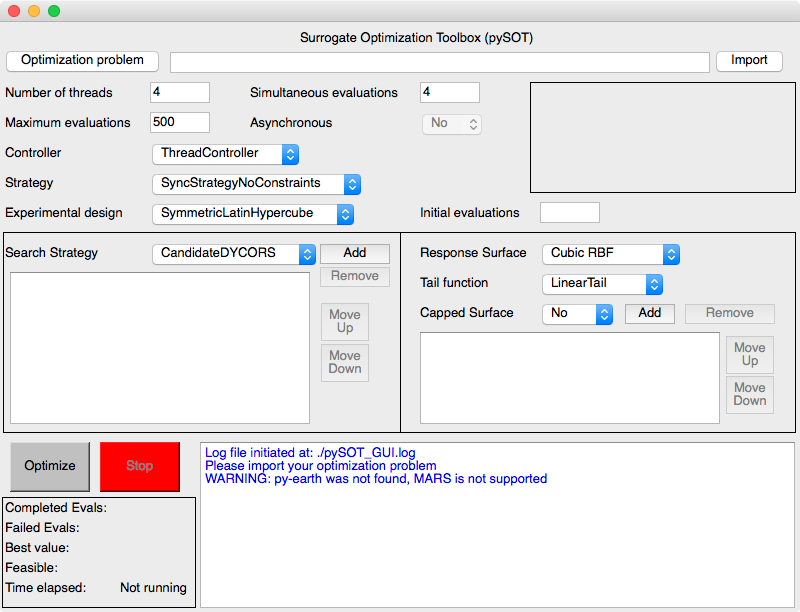
\includegraphics[width=\linewidth]{./Pics/GUI1}
                \caption{After initializing the GUI}
  \label{fig:First_figure}
       \end{subfigure}
    \hfill
        \begin{subfigure}{0.49\textwidth}\centering
                    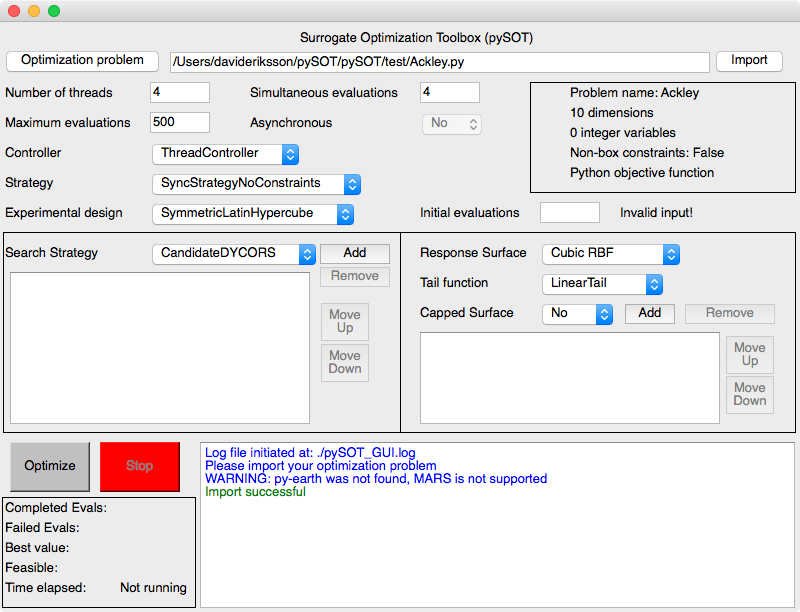
\includegraphics[width=\linewidth]{./Pics/GUI2}
                \caption{After importing an Optimization problem}
  \label{fig:Second_figure}
       \end{subfigure}%
    \hfill
        \begin{subfigure}{0.49\textwidth}\centering
                    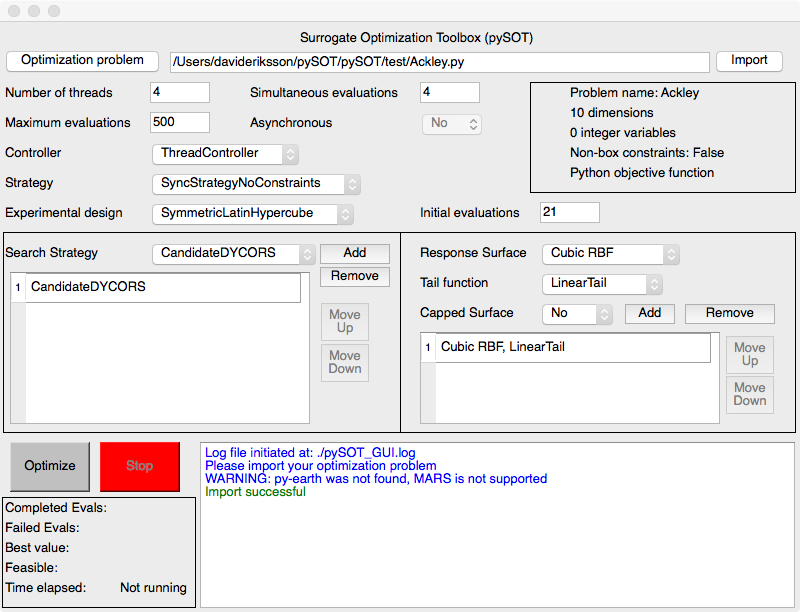
\includegraphics[width=\linewidth]{./Pics/GUI3}
                \caption{After choosing optimization components}
  \label{fig:Third_figure}
       \end{subfigure}%
    \hfill
        \begin{subfigure}{0.49\textwidth}\centering
                    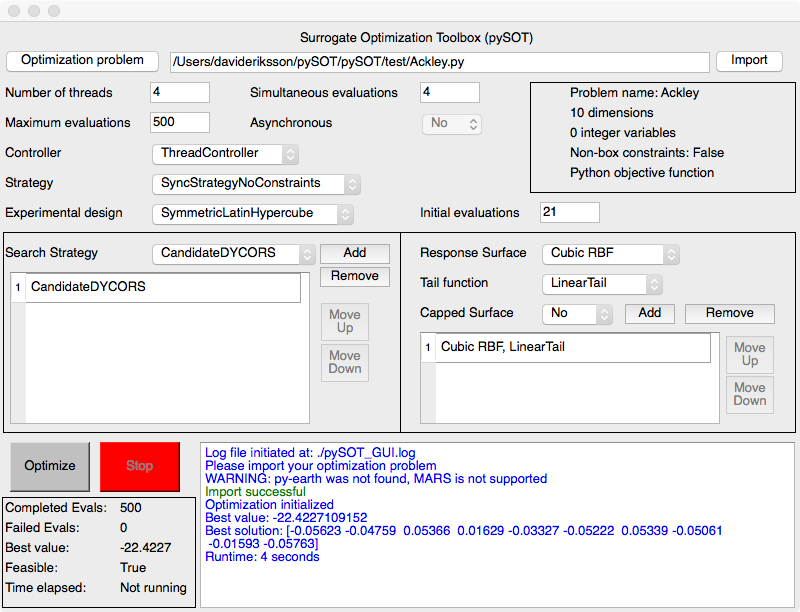
\includegraphics[width=\linewidth]{./Pics/GUI4}
                \caption{After running the optimizer}
  \label{fig:First_figure}
       \end{subfigure}%
       \caption{Illustration of the GUI}
 \label{fig:gui}
 \end{figure}
 
\section{Examples}
This section provides several examples that shows how to use POAP and pySOT to solve optimization problems.

\subsection{First example (Hello World)}
This example is a continuous optimization problem of the 10-dimensional Ackley-function which has only bound constraints. We are using 4 threads and 1000 evaluations. To generate new points to evaluate we use Candidate DyCORS. The experimental design is created using a Latin Hypercube with 2dim+1 points. The response surface is a cubic radial basis function with a linear tail. We use the ThreadController and the SyncStrategyNoConstraints strategy, since there are only bound constraints. We launch 4 BasicWorkerThread, start the optimization and finally print the result to the screen.

\begin{python}
import logging
from pySOT import *
from poap.controller import ThreadController, BasicWorkerThread
import numpy as np
import os.path

if not os.path.exists("./logfiles"):
    os.makedirs("logfiles")
logging.basicConfig(filename="./logfiles/test_simple.log",
                    level=logging.INFO)
print("Number of threads: 4")
print("Maximum number of evaluations: 1000")
print("Search strategy: Candidate DyCORS")
print("Experimental design: Latin Hypercube")
print("Ensemble surrogates: Cubic RBF")

nthreads = 4
maxeval = 1000
nsamples = nthreads

data = Ackley(dim=10)
print(data.info)

# Create a strategy and a controller
controller = ThreadController()
controller.strategy = \
    SyncStrategyNoConstraints(
        worker_id=0, data=data,
        maxeval=maxeval, nsamples=nsamples,
        exp_design=LatinHypercube(dim=data.dim, npts=2*data.dim+1),
        response_surface=RBFInterpolant(phi=phi_cubic, P=linear_tail,
                                        dphi=dphi_cubic, dP=dlinear_tail,
                                        eta=1e-8, maxp=maxeval),
        search_procedure=CandidateDyCORS(data=data, numcand=200*data.dim))

# Launch the threads and give them access to the objective function
for _ in range(nthreads):
    worker = BasicWorkerThread(controller, data.objfunction)
    controller.launch_worker(worker)

# Run the optimization strategy
result = controller.run()

print('Best value found: {0}'.format(result.value))
print('Best solution found: {0}'.format(
    np.array_str(result.params[0], max_line_width=np.inf,
                 precision=5, suppress_small=True)))
\end{python}

\subsection{Continuous problem with non-bound constraints}
This example is a continuous optimization problem of the 10-dimensional Keane's bump function which has two non-bound constraints. We are using 4 threads and 500 evaluations. To generate new points to evaluate we use Candidate DyCORS. The experimental design is created using a Latin Hypercube with 2dim+1 points. The response surface is a cubic radial basis function with a linear tail. We use the ThreadController and the SyncStrategyPenalty strategy, with the default penalty $10^6$. POAP doesn't check feasibility, so we need to modify the run command to supply a filter that makes POAP discard infeasible points when looking for the best solution at the end of the run. The feasible\_merit method simply sets infeasible points to have infinite function value so that only feasible points are considered. If for example small constraint violations are accepted the user can provide a merit function that is more suitable such a case.

\begin{python}
import logging
from pySOT import *
from poap.controller import ThreadController, BasicWorkerThread
import numpy as np
import os.path

if not os.path.exists("./logfiles"):
    os.makedirs("logfiles")
logging.basicConfig(filename="./logfiles/test_constraints.log",
                    level=logging.INFO)
print("Number of threads: 4")
print("Maximum number of evaluations: 500")
print("Search strategy: CandidateDycors")
print("Experimental design: Latin Hypercube")
print("Surrogate: Cubic RBF")

nthreads = 4
maxeval = 500
nsamples = nthreads

data = Keane(dim=10)
print(data.info)

def feasible_merit(record):
    """Merit function for ordering final answers -- kill infeasible x"""
    x = record.params[0].reshape((1, record.params[0].shape[0]))
    if np.max(data.eval_ineq_constraints(x)) > 0:
        return np.inf
    return record.value

# Create a strategy and a controller
controller = ThreadController()
controller.strategy = \
    SyncStrategyPenalty(
        worker_id=0, data=data,
        maxeval=maxeval, nsamples=nsamples,
        response_surface=RBFInterpolant(phi=phi_cubic, P=linear_tail,
                                        dphi=dphi_cubic, dP=dlinear_tail,
                                        eta=1e-8, maxp=maxeval),
        exp_design=LatinHypercube(dim=data.dim, npts=2*data.dim+1),
        search_procedure=CandidateDyCORS(data=data, numcand=5000))

# Launch the threads
for _ in range(nthreads):
    worker = BasicWorkerThread(controller, data.objfunction)
    controller.launch_worker(worker)

result = controller.run(merit=feasible_merit)
best, xbest = result.value, result.params[0]

print('Best value: {0}'.format(best))
print('Best solution: {0}'.format(
    np.array_str(xbest, max_line_width=np.inf,
                 precision=5, suppress_small=True)))
\end{python}

\subsection{Ensemble Surrogates}
This example is a continuous optimization problem of the 3-dimensional Hartman3-function which has only bound constraints. We are using 4 threads and 50 evaluations. To generate new points to evaluate we use Candidate SRBF, since the optimization problem is low-dimensional. The experimental design is created using a Latin Hypercube with 2dim+1 points. We also add the extra point [0.1, 0.5, 0.8], which we pretend is a known good solution to the problem. The response surface is an ensemble surrogate consisting of a cubic radial basis function with a linear tail, a linear radial basis function with constant tail, a thin-plate radial basis function with linear tail, and a MARS interpolant. We also redirect the stream from stdout and let pySOT print all messages to the text file surrogate\_optimizer.log placed in the current directory. We use the ThreadController and the SyncStrategyNoConstraints strategy, since there are only bound constraints. We launch 4 BasicWorkerThread, start the optimization and finally print the result to the screen.

\begin{python}
import logging
from pySOT import *
from poap.controller import ThreadController, BasicWorkerThread
import numpy as np
import os.path

if not os.path.exists("./logfiles"):
    os.makedirs("logfiles")
logging.basicConfig(filename="./logfiles/test_ensemble.log",
                    level=logging.INFO)
print("Number of threads: 4")
print("Maximum number of evaluations: 50")
print("Search strategy: Candidate SRBF")
print("Experimental design: Latin Hypercube + point [0.1, 0.5, 0.8]")
print("Surrogate: Cubic RBF, Linear RBF, Thin-plate RBF, MARS")

nthreads = 4
maxeval = 50
nsamples = nthreads

data = Hartman3()
print(data.info)

# Use 3 differents RBF's and MARS as an ensemble surrogate
models = [
    RBFInterpolant(phi_cubic, linear_tail, dphi_cubic,
                   dlinear_tail, 1e-8, maxeval),
    RBFInterpolant(phi_linear, const_tail, dphi_linear,
                   dconst_tail, 1e-8, maxeval),
    RBFInterpolant(dphi_plate, linear_tail, dphi_plate,
                   dlinear_tail, 1e-8, maxeval),
]
response_surface = EnsembleSurrogate(models, maxeval)

# Add an additional point to the experimental design. If a good
# solution is already known you can add this point to the
# experimental design
extra = np.atleast_2d([0.1, 0.5, 0.8])

# Create a strategy and a controller
controller = ThreadController()
controller.strategy = \
    SyncStrategyNoConstraints(
        worker_id=0, data=data,
        response_surface=response_surface,
        maxeval=maxeval, nsamples=nsamples,
        exp_design=LatinHypercube(dim=data.dim, npts=2*data.dim+1),
        search_procedure=CandidateSRBF(data=data, numcand=200*data.dim),
        extra=extra)

# Launch the threads and give them access to the objective function
for _ in range(nthreads):
    worker = BasicWorkerThread(controller, data.objfunction)
    controller.launch_worker(worker)

# Run the optimization strategy
result = controller.run()

response_surface.compute_weights()
print('Final weights: {0}'.format(
    np.array_str(response_surface.weights, max_line_width=np.inf,
                 precision=5, suppress_small=True)))

print('Best value found: {0}'.format(result.value))
print('Best solution found: {0}'.format(
    np.array_str(result.params[0], max_line_width=np.inf,
                 precision=5, suppress_small=True)))
\end{python}

\subsection{Mixed-integer problem with non-bound constraints}
This example is a mixed-integer optimization problem of a 5-dimensional problem with 3 inequality constraints. The first three variables are discrete and the last 2 are continuous. We are using 4 threads and 200 evaluations. To generate new points to evaluate we use a Multi-search strategy consisting of CandidateDyCORS, CandidateDyCORS\_INT, CandidateDyCORS\_CONT, and CandidateUniform. The experimental design is created using a Symmetric Latin Hypercube with 2dim+1 points. The response surface is a cubic radial basis function with a linear tail. We use the ThreadController and the SyncStrategyPenalty strategy, with the default penalty $10^6$. We submit the same merit function as in the previous example with constraints. The best solution is finally printed to the screen.

\begin{python}
import logging
from pySOT import *
from poap.controller import ThreadController, BasicWorkerThread
import numpy as np
import os.path

if not os.path.exists("./logfiles"):
    os.makedirs("logfiles")
logging.basicConfig(filename="./logfiles/test_mixed_integer_constraints.log",
                    level=logging.INFO)
print("Number of threads: 4")
print("Maximum number of evaluations: 200")
print("Search strategy: CandidateDyCORS, CandidateDyCORS_INT"
      ", CandidateDyCORS_CONT, CandidateUniform")
print("Experimental design: Symmetric Latin Hypercube")
print("Surrogate: Cubic RBF")

nthreads = 4
maxeval = 200
nsamples = nthreads

data = LinearMI()
print(data.info)

def feasible_merit(record):
    "Merit function for ordering final answers -- kill infeasible x"
    x = record.params[0].reshape((1, record.params[0].shape[0]))
    if np.max(data.eval_ineq_constraints(x)) > 0:
        return np.inf
    return record.value

exp_design = SymmetricLatinHypercube(dim=data.dim, npts=2*data.dim+1)
response_surface = RBFInterpolant(phi=phi_cubic, P=linear_tail,
                                  dphi=dphi_cubic, dP=dlinear_tail,
                                  eta=1e-8, maxp=maxeval)

# Use a multi-search strategy for candidate points
search_proc = MultiSearchStrategy(
    [CandidateDyCORS(data=data, numcand=200*data.dim),
     CandidateUniform(data=data, numcand=200*data.dim),
     CandidateDyCORS_INT(data=data, numcand=200*data.dim),
     CandidateDyCORS_CONT(data=data, numcand=200*data.dim)],
    [0, 1, 2, 3])

# Create a strategy and a controller
controller = ThreadController()
controller.strategy = \
    SyncStrategyPenalty( 
        worker_id=0, data=data,
        response_surface=response_surface,
        maxeval=maxeval, nsamples=nsamples,
        exp_design=exp_design,
        search_procedure=search_proc)

# Launch the threads
for _ in range(nthreads): 
    worker = BasicWorkerThread(controller, data.objfunction)
    controller.launch_worker(worker)

result = controller.run(merit=feasible_merit)
best, xbest = result.value, result.params[0]

print('Best value: {0}'.format(best))
print('Best solution: {0}'.format(
    np.array_str(xbest, max_line_width=np.inf,
                 precision=5, suppress_small=True)))
\end{python}

\subsection{External C++ objective function}
This last example shows how to use POAP and pySOT with an external objective function. We consider an objective function written in C++ that computes the sum of square of a given input, which is an easy convex optimization problem. The program takes its input as a string $'x_1,x_2,\ldots,x_n'$. With a probability of 0.9 the program prints the value of the sum of squares to the screen. With probability 0.1 the program prints nothing and terminates, which is supposed to imitate that the evaluation crashed. The C++ program that is compiled with the name sphere\_ext is provided below:
\lstset { %
    language=C++,
    backgroundcolor=\color{black!5}, % set backgroundcolor
    basicstyle=\footnotesize,% basic font setting
}
\begin{lstlisting}
#include <iostream>
#include <vector>
#include <sstream>
#include <unistd.h>
#include <numeric>
#include <random>

int main(int argc, char** argv) {
	// Random number generator
	std::random_device rand_dev;
	std::mt19937 generator(rand_dev());
	std::uniform_real_distribution<float>  distr(0.0, 1.0);

	// Pretend the simulation crashes with probability 0.1
  	if(distr(generator) > 0.1) {

		// Convert input to a standard vector
		std::vector<float> vect;
		std::stringstream ss(argv[1]);
		float f;

		while (ss >> f) {
    			vect.push_back(f);
			if (ss.peek() == ',')
    	    			ss.ignore();
		}
   		printf("%g\n", std::inner_product(vect.begin(), vect.end(), 
   	 				          vect.begin(), 0.0 ));
	}
	return 0;
}
\end{lstlisting}
We will use the subprocess library in Python to launch the objective function evaluations to our compiled C++ program. The help method array2str converts a numpy array to a string \textquotesingle$x_1,x_2,\ldots,x_n$\textquotesingle, which is what our C++ program wants as an input. The class SphereExt is the basic objective function class and the DummySim class overloads the evaluation method for a ProcessWorkerThread. In case the objective function evaluation fails, a message is printed to the screen just to illustrate that things are working correctly.

\lstset { %
    language=python,
    backgroundcolor=\color{white}, % set backgroundcolor
    basicstyle=\footnotesize,% basic font setting 
}
\begin{python}
import logging
from pySOT import *
from poap.controller import ThreadController, ProcessWorkerThread
import numpy as np
from subprocess import Popen, PIPE
import os.path

def array2str(x):
    return ",".join(np.char.mod('%f', x))


class SphereExt:
    def __init__(self, dim=10):
        self.xlow = -15 * np.ones(dim)
        self.xup = 20 * np.ones(dim)
        self.dim = dim
        self.info = str(dim)+"-dimensional Sphere function \n" + \
                    "Global optimum: f(0,0,...,0) = 0"
        self.min = 0
        self.integer = []
        self.continuous = np.arange(0, dim)


class DummySim(ProcessWorkerThread):

    def handle_eval(self, record):
        self.process = Popen(['./sphere_ext', array2str(record.params[0])],
                             stdout=PIPE)
        out = self.process.communicate()[0]
        try:
            val = float(out)  # This raises ValueError if out is not a float
            self.finish_success(record, val)
        except ValueError:
            logging.warning("Function evaluation crashed/failed")
            self.finish_failure(record)

if not os.path.exists("./logfiles"):
    os.makedirs("logfiles")
logging.basicConfig(filename="./logfiles/test_subprocess.log",
                    level=logging.INFO)

print("Number of threads: 4")
print("Maximum number of evaluations: 200")
print("Search strategy: Candidate DyCORS")
print("Experimental design: Latin Hypercube")
print("Ensemble surrogates: Cubic RBF")

assert os.path.isfile("./sphere_ext"), "You need to build sphere_ext"
nthreads = 4
maxeval = 200
nsamples = nthreads

data = SphereExt(dim=10)
print(data.info)

# Create a strategy and a controller
controller = ThreadController()
controller.strategy = \
    SyncStrategyNoConstraints(
        worker_id=0, data=data,
        maxeval=maxeval, nsamples=nsamples,
        exp_design=LatinHypercube(dim=data.dim, npts=2*data.dim+1),
        search_procedure=CandidateDyCORS(data=data, numcand=200*data.dim),
        response_surface=RBFInterpolant(phi=phi_cubic, P=linear_tail,
                                        dphi=dphi_cubic, dP=dlinear_tail,
                                        eta=1e-8, maxp=maxeval))

# Launch the threads and give them access to the objective function
for _ in range(nthreads):
    controller.launch_worker(DummySim(controller))

# Run the optimization strategy
result = controller.run()

print('Best value found: {0}'.format(result.value))
print('Best solution found: {0}'.format(
    np.array_str(result.params[0], max_line_width=np.inf,
                 precision=5, suppress_small=True)))
\end{python}

\section{Hierarchy of POAP + pySOT}
\begin{figure}[!ht] 
	\centering
	\resizebox{0.9\textwidth}{!}{ 
		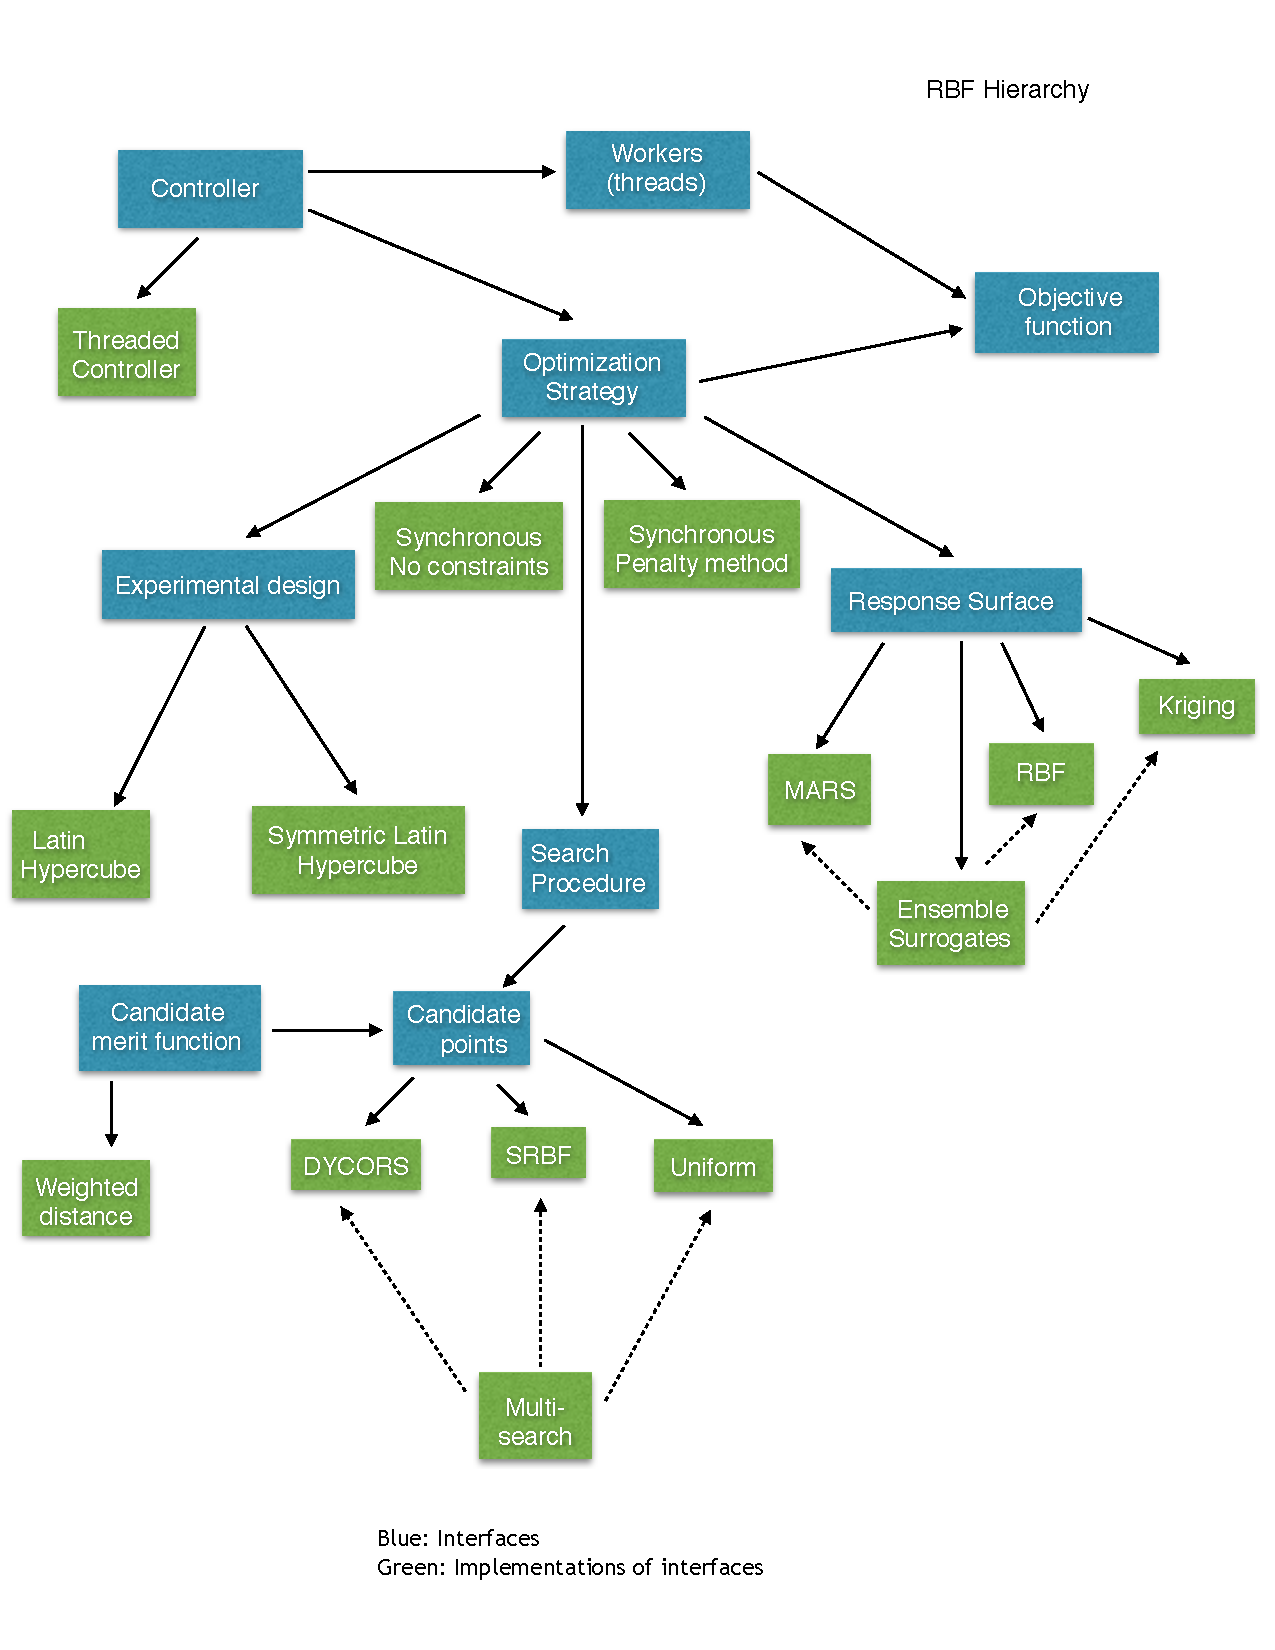
\includegraphics{RBFabstraction}} 
	\caption{Overview of the pySOT hierarchy} 
\end{figure}
\FloatBarrier

\section{Future changes}
\begin{itemize}
\item Add an asynchronous strategy
\item Add Heuristic Algorithms to search on the surrogate
\item Add more experimental designs
\item Add more methods for handling constraints, especially a barrier method
\item Support for Python 3.x
\end{itemize}
\end{document}
